% ==============================================================================
% Career Roadmap for AI Researchers: From Papers to Products
% SUNY Korea STEM Career Sprint 2026 — Yunsung Lee
% ==============================================================================

% ==============================================================================
% Paper2PR — Shared Beamer Preamble
% ==============================================================================
% Paper-agnostic preamble for all paper review presentations.
% Colors and environments match Quarto clean-academic.scss theme.
% ==============================================================================

\documentclass[aspectratio=169, 10pt]{beamer}

% --- Theme ---
\usetheme{default}
\usecolortheme{default}
\setbeamertemplate{navigation symbols}{}
\setbeamertemplate{footline}[frame number]
\setbeamertemplate{itemize items}[circle]
\setbeamertemplate{enumerate items}[default]

% --- Colors (matching Quarto clean-academic.scss) ---
\usepackage{xcolor}
\definecolor{primaryblue}{HTML}{012169}
\definecolor{primarygold}{HTML}{B9975B}
\definecolor{highlightyellow}{HTML}{F2A900}
\definecolor{lightbg}{HTML}{E8EDF5}
\definecolor{jet}{HTML}{1A1A1A}
\definecolor{positivegreen}{HTML}{15803D}
\definecolor{negativered}{HTML}{B91C1C}

\setbeamercolor{title}{fg=primaryblue}
\setbeamercolor{subtitle}{fg=primarygold}
\setbeamercolor{frametitle}{fg=primaryblue}
\setbeamercolor{structure}{fg=primaryblue}
\setbeamercolor{normal text}{fg=jet}
\setbeamercolor{itemize item}{fg=primaryblue}
\setbeamercolor{itemize subitem}{fg=primarygold}
\setbeamercolor{enumerate item}{fg=highlightyellow}

% --- Fonts (XeLaTeX) ---
\usepackage{fontspec}
% Source Sans Pro (static OTF from TexLive — explicit path for reliability)
\setsansfont{SourceSansPro}[
  Path = /usr/local/texlive/2024/texmf-dist/fonts/opentype/adobe/sourcesanspro/,
  UprightFont = SourceSansPro-Regular.otf,
  BoldFont = SourceSansPro-Bold.otf,
  ItalicFont = SourceSansPro-RegularIt.otf,
  BoldItalicFont = SourceSansPro-BoldIt.otf,
  Scale = 1.0
]
\usefonttheme{professionalfonts}

% --- Math ---
\usepackage{amsmath}
\usepackage{amssymb}
\usepackage{bm}
\usepackage{mathtools}

% --- Graphics ---
\usepackage{graphicx}
\usepackage{tikz}
\usepackage{booktabs}
\usepackage{multicol}
\usepackage{hyperref}

% --- tcolorbox for custom environments ---
\usepackage[most]{tcolorbox}

% methodbox — Blue-bordered for technical details
\newtcolorbox{methodbox}[1][]{%
  colback=primaryblue!6,
  colframe=primaryblue,
  coltitle=white,
  fonttitle=\bfseries,
  left=8pt, right=8pt, top=6pt, bottom=6pt,
  boxrule=0pt, leftrule=4pt,
  arc=4pt,
  title={#1}
}

% keybox — Gold-bordered for key insights
\newtcolorbox{keybox}[1][]{%
  colback=primarygold!12,
  colframe=primarygold,
  coltitle=white,
  fonttitle=\bfseries,
  left=8pt, right=8pt, top=6pt, bottom=6pt,
  boxrule=0pt, leftrule=4pt,
  arc=4pt,
  title={#1}
}

% highlightbox — Yellow-bordered for notable findings
\newtcolorbox{highlightbox}[1][]{%
  colback=highlightyellow!8,
  colframe=highlightyellow,
  coltitle=white,
  fonttitle=\bfseries,
  left=8pt, right=8pt, top=6pt, bottom=6pt,
  boxrule=0pt, leftrule=4pt,
  arc=4pt,
  title={#1}
}

% assumptionbox — Gold full-border for assumptions
\newtcolorbox{assumptionbox}[1][]{%
  colback=primarygold!8,
  colframe=primarygold,
  coltitle=white,
  fonttitle=\bfseries,
  left=8pt, right=8pt, top=6pt, bottom=6pt,
  boxrule=2pt,
  arc=4pt,
  title={#1}
}

% resultbox — Gold-bordered with shadow for main results
\newtcolorbox{resultbox}[1][]{%
  colback=primarygold!15,
  colframe=primarygold,
  coltitle=white,
  fonttitle=\bfseries,
  left=8pt, right=8pt, top=6pt, bottom=6pt,
  boxrule=2pt,
  arc=4pt,
  shadow={1pt}{-1pt}{0pt}{black!12},
  title={#1}
}

% eqbox — Subtle blue background for equations
\newtcolorbox{eqbox}{%
  colback=primaryblue!4,
  colframe=primaryblue!4,
  left=8pt, right=8pt, top=4pt, bottom=4pt,
  boxrule=0pt,
  arc=0pt
}

% softbox — Subtle gold italic for remarks
\newtcolorbox{softbox}{%
  colback=primarygold!6,
  colframe=primarygold!6,
  left=8pt, right=8pt, top=4pt, bottom=4pt,
  boxrule=0pt,
  arc=0pt,
  fontupper=\itshape
}

% quotebox — Italic with decorative quote mark
\newtcolorbox{quotebox}{%
  colback=primarygold!8,
  colframe=primarygold!80!black,
  left=16pt, right=8pt, top=6pt, bottom=6pt,
  boxrule=0pt, leftrule=4pt,
  arc=0pt, outer arc=4pt,
  fontupper=\itshape,
  before upper={\textcolor{primarygold!40}{\Large``}\,}
}

% --- Text color commands ---
\newcommand{\hi}[1]{{\bfseries\color{primaryblue}#1}}
\newcommand{\higold}[1]{{\bfseries\color{primarygold}#1}}
\newcommand{\hiyellow}[1]{{\bfseries\color{highlightyellow}#1}}
\newcommand{\higreen}[1]{{\bfseries\color{positivegreen}#1}}
\newcommand{\hired}[1]{{\bfseries\color{negativered}#1}}
\newcommand{\positive}[1]{{\bfseries\color{positivegreen}#1}}
\newcommand{\negative}[1]{{\bfseries\color{negativered}#1}}
\newcommand{\neutral}[1]{{\color{gray}#1}}

% --- Bibliography ---
\usepackage[
  backend=bibtex,
  style=authoryear,
  natbib=true,
  maxcitenames=2
]{biblatex}

% --- Title page template (compact, no internal \vfill) ---
\setbeamertemplate{title page}{
  \begin{center}
    \vspace{1em}
    {\Large\bfseries\color{primaryblue}\inserttitle}

    \vspace{0.4em}
    {\normalsize\color{primarygold}\insertsubtitle}

    \vspace{0.8em}
    {\normalsize\insertauthor}

    \vspace{0.2em}
    {\small\textcolor{primarygold}{\insertinstitute}}
  \end{center}
}

% --- Frame title formatting ---
\setbeamerfont{frametitle}{size=\large, series=\bfseries}
\setbeamertemplate{frametitle}{%
  \vspace{0.3em}
  \insertframetitle
  \vspace{0.1em}
  {\color{primarygold!30}\hrule height 2pt}
}

\usepackage{pgfplots}
\pgfplotsset{compat=1.18}
\usetikzlibrary{positioning}
\usepackage[normalem]{ulem}
\addbibresource{../Bibliography_base.bib}

\title{Career Roadmap for AI Researchers\\From Papers to Products}
\subtitle{SUNY Korea STEM Career Sprint 2026}
\author{Yunsung Lee}
\institute{WoRV / Maum.ai}
\date{April 4, 2026}

\begin{document}

% ==============================================================================
% PART 0: OPENING (slides 1–3)
% ==============================================================================

% --- Slide 1: Title ---
\begin{frame}[plain]
\maketitle
\vspace{1.2em}
\begin{center}
  {\small\color{primarygold}
    Stories from a Physical AI Research Lead \& a 5M-User AI Agent Builder}
\end{center}
\end{frame}

% --- Slide 2: Who Am I? ---
\begin{frame}{Who Am I?}
\begin{columns}[T]
  \begin{column}{0.55\textwidth}
    \vspace{0.3em}
    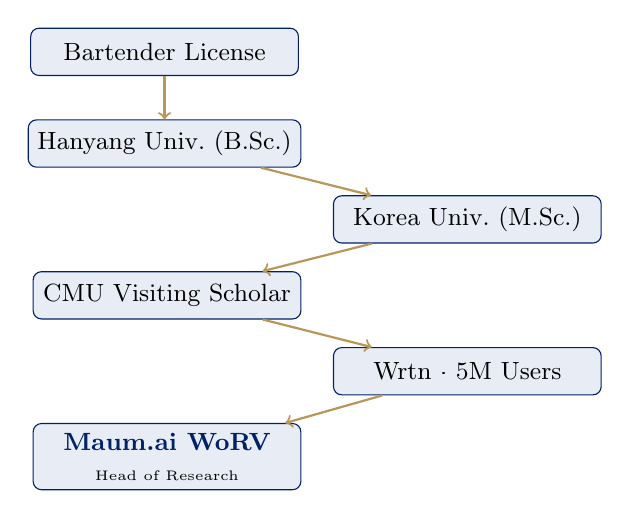
\begin{tikzpicture}[
      node distance=0.55cm,
      box/.style={draw=primaryblue, rounded corners=3pt, fill=lightbg,
                  minimum width=3.4cm, minimum height=0.6cm,
                  font=\small, align=center},
      arrow/.style={->, thick, color=primarygold}
    ]
      \node[box] (bar)  {Bartender License};
      \node[box, below=of bar]  (han)  {Hanyang Univ.\ (B.Sc.)};
      \node[box, below right=0.35cm and 0.4cm of han] (kor)  {Korea Univ.\ (M.Sc.)};
      \node[box, below left=0.35cm and 0.4cm of kor]  (cmu)  {CMU Visiting Scholar};
      \node[box, below right=0.35cm and 0.4cm of cmu] (wrtn) {Wrtn · 5M Users};
      \node[box, below left=0.35cm and 0.4cm of wrtn] (maum) {\hi{Maum.ai WoRV}\\
            \tiny Head of Research};

      \draw[arrow] (bar)  -- (han);
      \draw[arrow] (han)  -- (kor);
      \draw[arrow] (kor)  -- (cmu);
      \draw[arrow] (cmu)  -- (wrtn);
      \draw[arrow] (wrtn) -- (maum);
    \end{tikzpicture}
  \end{column}
  \begin{column}{0.42\textwidth}
    \vspace{1.5em}
    \begin{center}
      {\fontsize{36}{40}\selectfont\hi{10+}}\\[0.15em]
      {\small Papers (ICLR, CVPR, NeurIPS)}\\[1.4em]
      {\fontsize{36}{40}\selectfont\higold{1,844}}\\[0.15em]
      {\small Citations (Google Scholar)}
    \end{center}
    \vspace{1em}
    \begin{keybox}[]
      \footnotesize Non-linear path. Intentional.
    \end{keybox}
  \end{column}
\end{columns}
\end{frame}

% --- Slide 3: What You'll Walk Away With ---
\begin{frame}{What You'll Walk Away With}
\vspace{0.5em}
\begin{columns}[c]
  \begin{column}{0.24\textwidth}
    \begin{center}
      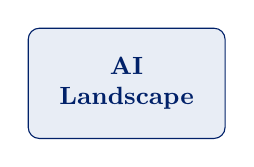
\begin{tikzpicture}
        \node[draw=primaryblue, fill=lightbg, rounded corners=4pt,
              minimum width=2.5cm, minimum height=1.4cm,
              align=center, font=\small\bfseries\color{primaryblue}]
              {AI\\Landscape};
      \end{tikzpicture}\\[0.3em]
      {\footnotesize\neutral{\$245K median}}
    \end{center}
  \end{column}
  \begin{column}{0.24\textwidth}
    \begin{center}
      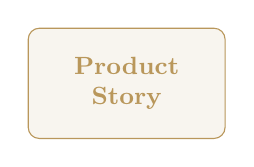
\begin{tikzpicture}
        \node[draw=primarygold, fill=primarygold!10, rounded corners=4pt,
              minimum width=2.5cm, minimum height=1.4cm,
              align=center, font=\small\bfseries\color{primarygold}]
              {Product\\Story};
      \end{tikzpicture}\\[0.3em]
      {\footnotesize\neutral{5M+ MAU}}
    \end{center}
  \end{column}
  \begin{column}{0.24\textwidth}
    \begin{center}
      
\begin{tikzpicture}
        \node[draw=primaryblue, fill=lightbg, rounded corners=4pt,
              minimum width=2.5cm, minimum height=1.4cm,
              align=center, font=\small\bfseries\color{primaryblue}]
              {Research\\Story};
      \end{tikzpicture}\\[0.3em]
      {\footnotesize\neutral{97.3\% success}}
    \end{center}
  \end{column}
  \begin{column}{0.24\textwidth}
    \begin{center}
      
\begin{tikzpicture}
        \node[draw=primarygold, fill=primarygold!10, rounded corners=4pt,
              minimum width=2.5cm, minimum height=1.4cm,
              align=center, font=\small\bfseries\color{primarygold}]
              {Your Action\\Plan};
      \end{tikzpicture}\\[0.3em]
      {\footnotesize\neutral{Start today}}
    \end{center}
  \end{column}
\end{columns}
\vspace{1.4em}
\begin{center}
  {\large\hi{3 real stories.} \higold{Concrete numbers.} A career plan you can start today.}
\end{center}
\end{frame}

% ==============================================================================
% PART 1: THE AI CAREER LANDSCAPE IN 2026 (slides 4–11)
% ==============================================================================

% --- Slide 4: AI Changed Everything ---
\begin{frame}{AI Changed Everything}
\begin{center}
  {\fontsize{48}{56}\selectfont\hi{200,000,000}}\\[0.4em]
  {\large ChatGPT users.\quad Two years.}\\[1em]
  {\normalsize The entire industry restructured around this number.}\\[1.4em]
  \begin{columns}[t]
    \begin{column}{0.45\textwidth}
      \begin{highlightbox}[Before (2022)]
        \footnotesize Software Engineer · Data Scientist\\
        DevOps · Product Manager
      \end{highlightbox}
    \end{column}
    \begin{column}{0.45\textwidth}
      \begin{keybox}[After (2024--2026)]
        \footnotesize \hi{AI Engineer} · \hi{MLOps Engineer}\\
        \hi{AI PM} · \hi{AI Safety Researcher}
      \end{keybox}
    \end{column}
  \end{columns}
\end{center}
\vspace{0.6em}
{\footnotesize\neutral{Source: OpenAI Feb 2025; LinkedIn Jobs on the Rise 2026; WEF Future of Jobs 2025}}
\end{frame}

% --- Slide 5: The AI Job Map ---
\begin{frame}{The AI Job Map}
\begin{center}
  {\small\hi{4 Paths.}\quad Researcher / Engineer / PM / Data.\quad Know the difference before you apply.}
\end{center}
\vspace{0.5em}
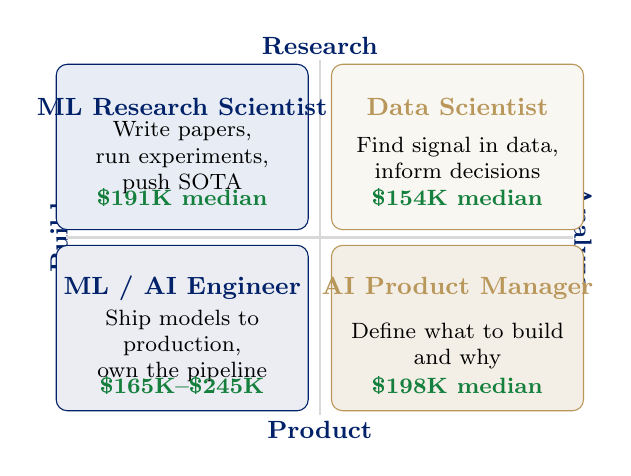
\begin{tikzpicture}[scale=0.92]
  % Axes labels
  \node[font=\small\bfseries\color{primaryblue}] at (3.5, 5.1)  {Research};
  \node[font=\small\bfseries\color{primaryblue}] at (3.5, -0.2) {Product};
  \node[font=\small\bfseries\color{primaryblue}] at (-0.1, 2.45) [rotate=90] {Build};
  \node[font=\small\bfseries\color{primaryblue}] at (7.1,  2.45) [rotate=270] {Analyze};

  % Grid lines
  \draw[gray!30, thick] (0,2.45) -- (7, 2.45);
  \draw[gray!30, thick] (3.5,0)  -- (3.5, 4.9);

  % Quadrant: Research + Build (top-left)
  \node[draw=primaryblue, fill=lightbg, rounded corners=4pt,
        minimum width=3.2cm, minimum height=2.1cm, align=center]
        at (1.6, 3.7) {};
  \node[font=\small\bfseries\color{primaryblue}, align=center]
        at (1.6, 4.25) {ML Research Scientist};
  \node[font=\footnotesize, align=center, text width=2.8cm]
        at (1.6, 3.55) {Write papers, run experiments,\\push SOTA};
  \node[font=\footnotesize\bfseries\color{positivegreen}]
        at (1.6, 3.0) {\$191K median};

  % Quadrant: Research + Analyze (top-right)
  \node[draw=primarygold, fill=primarygold!8, rounded corners=4pt,
        minimum width=3.2cm, minimum height=2.1cm, align=center]
        at (5.4, 3.7) {};
  \node[font=\small\bfseries\color{primarygold}, align=center]
        at (5.4, 4.25) {Data Scientist};
  \node[font=\footnotesize, align=center, text width=2.8cm]
        at (5.4, 3.55) {Find signal in data,\\inform decisions};
  \node[font=\footnotesize\bfseries\color{positivegreen}]
        at (5.4, 3.0) {\$154K median};

  % Quadrant: Product + Build (bottom-left)
  \node[draw=primaryblue, fill=primaryblue!8, rounded corners=4pt,
        minimum width=3.2cm, minimum height=2.1cm, align=center]
        at (1.6, 1.2) {};
  \node[font=\small\bfseries\color{primaryblue}, align=center]
        at (1.6, 1.75) {ML / AI Engineer};
  \node[font=\footnotesize, align=center, text width=2.8cm]
        at (1.6, 0.95) {Ship models to production,\\own the pipeline};
  \node[font=\footnotesize\bfseries\color{positivegreen}]
        at (1.6, 0.4) {\$165K--\$245K};

  % Quadrant: Product + Analyze (bottom-right)
  \node[draw=primarygold, fill=primarygold!15, rounded corners=4pt,
        minimum width=3.2cm, minimum height=2.1cm, align=center]
        at (5.4, 1.2) {};
  \node[font=\small\bfseries\color{primarygold}, align=center]
        at (5.4, 1.75) {AI Product Manager};
  \node[font=\footnotesize, align=center, text width=2.8cm]
        at (5.4, 0.95) {Define what to build\\and why};
  \node[font=\footnotesize\bfseries\color{positivegreen}]
        at (5.4, 0.4) {\$198K median};
\end{tikzpicture}
\end{frame}

% --- Slide 6: Salary Reality Check ---
\begin{frame}{Salary Reality Check}
\begin{center}
  {\large\hi{\$245,000}}\quad US median total comp for AI engineers.\\[0.2em]
  {\normalsize Korea? \higold{6\% premium} over non-AI. That gap is not a rumor.}
\end{center}
\vspace{0.6em}
\begin{columns}[b]
  \begin{column}{0.48\textwidth}
    \begin{center}
      {\small\bfseries United States}\\[0.3em]
      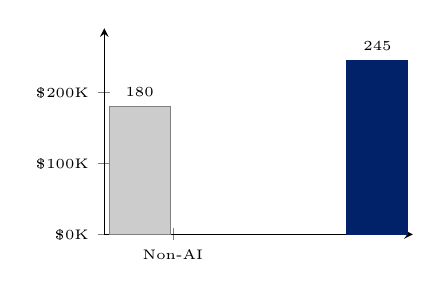
\begin{tikzpicture}
        \begin{axis}[
          ybar, bar width=22pt,
          width=5.5cm, height=4.2cm,
          symbolic x coords={Non-AI, AI},
          xtick=data,
          ymin=0, ymax=290,
          ytick={0,100,200},
          yticklabels={\$0K,\$100K,\$200K},
          tick label style={font=\tiny},
          axis lines=left,
          enlarge x limits=0.4,
          nodes near coords,
          nodes near coords style={font=\tiny\bfseries},
          every node near coord/.append style={/pgf/number format/.cd, fixed, precision=0},
        ]
          \addplot[fill=gray!40, draw=gray] coordinates {(Non-AI,180)};
          \addplot[fill=primaryblue, draw=primaryblue] coordinates {(AI,245)};
        \end{axis}
      \end{tikzpicture}\\[0.2em]
      {\footnotesize\positive{+36\% premium at median}}
    \end{center}
  \end{column}
  \begin{column}{0.48\textwidth}
    \begin{center}
      {\small\bfseries Korea}\\[0.3em]
      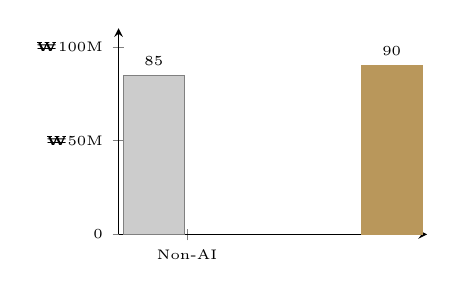
\begin{tikzpicture}
        \begin{axis}[
          ybar, bar width=22pt,
          width=5.5cm, height=4.2cm,
          symbolic x coords={Non-AI, AI},
          xtick=data,
          ymin=0, ymax=110,
          ytick={0,50,100},
          yticklabels={0,\textbf{₩}50M,\textbf{₩}100M},
          tick label style={font=\tiny},
          axis lines=left,
          enlarge x limits=0.4,
          nodes near coords,
          nodes near coords style={font=\tiny\bfseries},
          every node near coord/.append style={/pgf/number format/.cd, fixed, precision=0},
        ]
          \addplot[fill=gray!40, draw=gray] coordinates {(Non-AI,85)};
          \addplot[fill=primarygold, draw=primarygold] coordinates {(AI,90)};
        \end{axis}
      \end{tikzpicture}\\[0.2em]
      {\footnotesize\neutral{+6\% premium}}
    \end{center}
  \end{column}
\end{columns}
\vspace{0.3em}
{\footnotesize\neutral{Source: Levels.fyi Q3 2025; Korea wage data 2025. Values in USD / KRW approximate.}}
\end{frame}

% --- Slide 7: The Paradox ---
\begin{frame}{The Paradox}
\vspace{0.4em}
\begin{columns}[c]
  \begin{column}{0.44\textwidth}
    \begin{center}
      {\fontsize{52}{58}\selectfont\negative{50\%}}\\[0.3em]
      {\normalsize\bfseries AI/ML positions unfilled}\\[0.2em]
      {\footnotesize\neutral{92\% increase in AI hiring demand}}
    \end{center}
  \end{column}
  \begin{column}{0.10\textwidth}
    \begin{center}
      {\Large\bfseries\color{primarygold} WHY?}
    \end{center}
  \end{column}
  \begin{column}{0.44\textwidth}
    \begin{center}
      {\fontsize{52}{58}\selectfont\hi{6.1\%}}\\[0.3em]
      {\normalsize\bfseries CS graduates unemployed (2025)}\\[0.2em]
      {\footnotesize\neutral{CS ranks 7th highest unemployment\\among all college majors}}
    \end{center}
  \end{column}
\end{columns}
\vspace{1.2em}
\begin{highlightbox}[]
  \centering
  {\bfseries Skills mismatch.}
  The market wants AI specialists who ship. It does not want generalists.
\end{highlightbox}
\end{frame}

% --- Slide 8: What the Market Actually Wants ---
\begin{frame}{What the Market Actually Wants}
\begin{center}
  {\large \negative{Not your GPA.}\quad \negative{Not your degree.}\quad \hi{Your ability to ship.}}
\end{center}
\vspace{0.2em}
\begin{tabular}{p{4.8cm} p{5.8cm}}
  \toprule
  \textbf{\neutral{What You Think They Want}} & \textbf{\hi{What They Actually Hire For}} \\
  \midrule
  High GPA & Portfolio projects \higold{(38\% of tech leaders)} \\[3pt]
  Prestigious university & Internship experience \higold{(35\%)} \\[3pt]
  Certifications \& courses & Public code / GitHub contributions \higold{(34\%)} \\[3pt]
  Knowing all the math & Can you ship end-to-end? \\[3pt]
  Publications (for eng.\ roles) & Deployed projects with real users \\[3pt]
  Long skills list & Depth in 2--3 areas + proof \\
  \bottomrule
\end{tabular}
\vspace{0.2em}
\begin{keybox}[]
  \centering
  \footnotesize Only \higold{4\%} of hiring leaders cited credentials.\quad
  Only \higold{17\%} cited school prestige.\\
  \neutral{Source: Fortune Tech Hiring Secrets, Dec 2025}
\end{keybox}
\end{frame}

% --- Slide 9: Physical AI: The Next Frontier ---
\begin{frame}{Physical AI: The Next Frontier}
\begin{columns}[T]
  \begin{column}{0.52\textwidth}
    \begin{center}
      {\large\hi{\$6B+}}\quad VC into robotics, H1 2025 alone.\\[0.1em]
      {\footnotesize\neutral{More than all of 2024 (\$6.1B full year).}}\\[0.5em]
      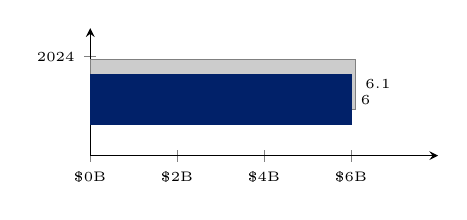
\begin{tikzpicture}
        \begin{axis}[
          xbar, bar width=18pt,
          width=6cm, height=3.2cm,
          symbolic y coords={H1 2025, 2024},
          ytick=data,
          xmin=0, xmax=8,
          xtick={0,2,4,6},
          xticklabels={\$0B,\$2B,\$4B,\$6B},
          tick label style={font=\tiny},
          axis lines=left,
          enlarge y limits=0.4,
          nodes near coords,
          nodes near coords align=horizontal,
          nodes near coords style={font=\tiny\bfseries},
        ]
          \addplot[fill=gray!40, draw=gray] coordinates {(6.1,2024)};
          \addplot[fill=primaryblue, draw=primaryblue] coordinates {(6.0,{H1 2025})};
        \end{axis}
      \end{tikzpicture}
    \end{center}
  \end{column}
  \begin{column}{0.45\textwidth}
    \vspace{0.3em}
    {\footnotesize
    \begin{tabular}{ll}
      \toprule
      \multicolumn{2}{l}{\small\bfseries Key Players} \\
      \midrule
      NVIDIA & Isaac GR00T \\
      Figure AI & \$39B valuation \\
      Tesla & Optimus \\
      Google DeepMind & Gemini Robotics \\
      Hyundai & Boston Dynamics \\
      \bottomrule
    \end{tabular}
    }
    \vspace{0.5em}
    \begin{keybox}[]
      \footnotesize\centering
      \hi{Korea:} 60\% of CES 2026\\
      Innovation Awards\\
      \neutral{(168 of 284 companies)}
    \end{keybox}
  \end{column}
\end{columns}
\vspace{0.2em}
{\footnotesize\neutral{Source: Crunchbase 2025; Marion Street Capital; KoreaTechDesk CES 2026}}
\end{frame}

% --- Slide 10: Korea's ₩10.1 Trillion AI Bet ---
\begin{frame}{Korea's ₩10.1 Trillion AI Bet}
\begin{center}
  {\fontsize{52}{58}\selectfont\hi{₩10.1T}}\\[0.4em]
  {\large Korea's 2026 AI national budget.}\\[0.2em]
  {\normalsize\higold{206\% increase} from 2025.}\\[0.6em]
  \begin{columns}[t]
    \begin{column}{0.3\textwidth}
      \begin{methodbox}[Government]
        \footnotesize ₩200B for 5 sovereign AI\\
        foundation models\\[2pt]
        Manufacturing AI (M.AX):\\
        ₩700B in 2026
      \end{methodbox}
    \end{column}
    \begin{column}{0.3\textwidth}
      \begin{resultbox}[Industry]
        \footnotesize Samsung + SK + Hyundai\\
        \hi{₩703T} combined\\
        investment pledge
      \end{resultbox}
    \end{column}
    \begin{column}{0.35\textwidth}
      {\footnotesize\higold{Ecosystem}}\\[0.3em]
      \footnotesize Seoul: \higold{\#2 global AI city}\\
      (Counterpoint Research 2025)\\[2pt]
      45.5\% of Q3 2025 funded\\
      Korean startups are AI
    \end{column}
  \end{columns}
\end{center}
\vspace{0.3em}
{\footnotesize\neutral{1 USD \(\approx\) 1,400 KRW for context}}
\end{frame}

% --- Slide 11: Two Paths I Took ---
\begin{frame}{Two Paths I Took}
\vspace{0.3em}
\begin{center}
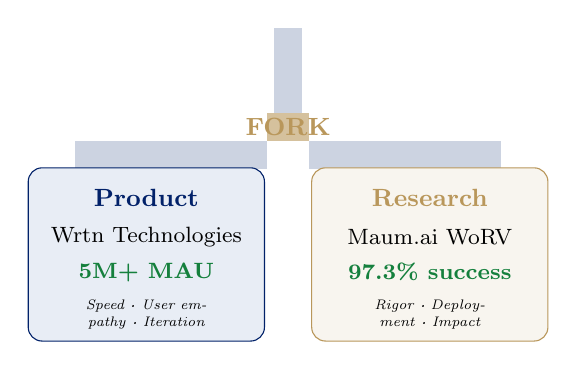
\begin{tikzpicture}[scale=0.9]
  % The single road coming in from top
  \fill[primaryblue!20] (3.3,4.8) -- (3.7,4.8) -- (3.7,3.6) -- (3.3,3.6) -- cycle;

  % Fork point
  \fill[primarygold!60] (3.2,3.6) -- (3.8,3.6) -- (3.8,3.2) -- (3.2,3.2) -- cycle;

  % Left road (Product)
  \fill[primaryblue!20] (0.5,3.2) -- (3.2,3.2) -- (3.2,2.8) -- (0.5,2.8) -- cycle;

  % Right road (Research)
  \fill[primaryblue!20] (3.8,3.2) -- (6.5,3.2) -- (6.5,2.8) -- (3.8,2.8) -- cycle;

  % Left path box
  \node[draw=primaryblue, fill=lightbg, rounded corners=5pt,
        minimum width=3.0cm, minimum height=2.2cm, align=center]
        at (1.5, 1.6) {};
  \node[font=\small\bfseries\color{primaryblue}] at (1.5, 2.4)   {Product};
  \node[font=\footnotesize, align=center]        at (1.5, 1.85)   {Wrtn Technologies};
  \node[font=\footnotesize\bfseries\color{positivegreen}, align=center]
                                                  at (1.5, 1.35) {5M+ MAU};
  \node[font=\tiny\itshape, align=center, text width=2.6cm]
                                                  at (1.5, 0.75) {Speed · User empathy · Iteration};

  % Right path box
  \node[draw=primarygold, fill=primarygold!10, rounded corners=5pt,
        minimum width=3.0cm, minimum height=2.2cm, align=center]
        at (5.5, 1.6) {};
  \node[font=\small\bfseries\color{primarygold}] at (5.5, 2.4)   {Research};
  \node[font=\footnotesize, align=center]        at (5.5, 1.85)   {Maum.ai WoRV};
  \node[font=\footnotesize\bfseries\color{positivegreen}, align=center]
                                                  at (5.5, 1.35) {97.3\% success};
  \node[font=\tiny\itshape, align=center, text width=2.6cm]
                                                  at (5.5, 0.75) {Rigor · Deployment · Impact};

  % Labels
  \node[font=\small\bfseries\color{primarygold}] at (3.5, 3.4) {FORK};
\end{tikzpicture}
\end{center}
\vspace{0.3em}
\begin{keybox}[]
  \centering
  {\small Both roads converge on one skill:\quad \hi{knowing what problem to solve.}}
\end{keybox}
\end{frame}

% ==============================================================================
% PART 2: MY WRTN STORY — BUILDING A 5M-USER AI AGENT (slides 12–23)
% ==============================================================================

% --- Section Divider ---
\begin{frame}[plain]
\begin{center}
\vfill
{\Huge\hi{Building a 5M-User AI Agent}}\\[1em]
{\large\higold{My Wrtn Story}}
\vfill
\end{center}
\end{frame}

% --- Slide 12: Wrtn Technologies ---
\begin{frame}{Wrtn Technologies}
\begin{center}
  {\large Korea's \hi{\#1} AI-native startup.}\\[0.8em]
  {\normalsize\itshape I joined when the stakes were highest.}\\[1.4em]
  \begin{methodbox}[]
    \centering
    {\small Seoul\ \textperiodcentered\ Founded 2022\ \textperiodcentered\
    Oct 2023--Apr 2025: Yunsung Lee, AI Engineer}
  \end{methodbox}
  \vspace{0.8em}
  {\normalsize Korea's most-used AI productivity platform.}\\[0.3em]
  {\footnotesize\neutral{``My Own AI'' — a personal assistant that actually knows you.}}
\end{center}
\end{frame}

% --- Slide 13: 5M+ Users Hero Stat ---
\begin{frame}{"My Own AI" — 5M+ Users}
\begin{center}
  \vspace{0.6em}
  {\fontsize{64}{72}\selectfont\hi{5,000,000+}}\\[0.5em]
  {\large Monthly Active Users}\\[1.2em]
  {\normalsize\itshape I owned this product end-to-end.}\\[1em]
  {\footnotesize\neutral{My Own AI autonomous agent · Wrtn Technologies · 2023--2025}}
\end{center}
\end{frame}

% --- Slide 14: Memory & Personalization RAG ---
\begin{frame}{Memory \& Personalization RAG}
\begin{columns}[T]
  \begin{column}{0.47\textwidth}
    \begin{highlightbox}[Before: Generic AI]
      \footnotesize\centering
      {\color{gray}``How can I help you today?''}\\[0.3em]
      \neutral{No memory. No context.\\Starts from zero every session.}
    \end{highlightbox}
  \end{column}
  \begin{column}{0.47\textwidth}
    \begin{keybox}[After: Personalized AI]
      \footnotesize\centering
      \hi{``Good morning — your presentation}\\
      \hi{is today. Want help with the opening?''}\\[0.3em]
      \positive{Remembers. Anticipates. Personalizes.}
    \end{keybox}
  \end{column}
\end{columns}
\vspace{1em}
\begin{center}
  {\fontsize{40}{46}\selectfont\positive{+12.7\%}}\\[0.3em]
  {\normalsize Week-1 Retention Lift}\\[0.5em]
  {\small\itshape Memory changed everything.}
\end{center}
\end{frame}

% --- Slide 15: Real-time Web Search RAG ---
\begin{frame}{Real-time Web Search RAG}
\begin{center}
  {\normalsize\itshape ``What's the weather in Busan?''\ \ The AI had to \hi{actually know}.}
\end{center}
\vspace{0.8em}
\begin{center}
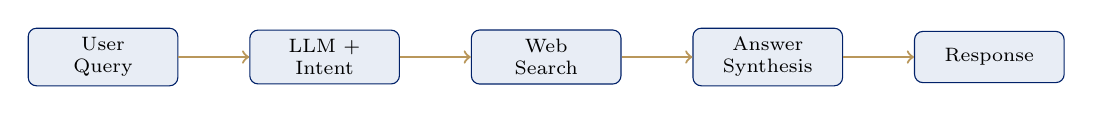
\begin{tikzpicture}[
  node distance=0.9cm,
  box/.style={draw=primaryblue, fill=lightbg, rounded corners=3pt,
              minimum width=1.9cm, minimum height=0.65cm,
              font=\scriptsize, align=center},
  arr/.style={->, thick, color=primarygold}
]
  \node[box] (q)   {User\\Query};
  \node[box, right=of q]  (c)   {LLM +\\Intent};
  \node[box, right=of c]  (ws)  {Web\\Search};
  \node[box, right=of ws] (syn) {Answer\\Synthesis};
  \node[box, right=of syn](r)   {Response};

  \draw[arr] (q)   -- (c);
  \draw[arr] (c)   -- (ws);
  \draw[arr] (ws)  -- (syn);
  \draw[arr] (syn) -- (r);
\end{tikzpicture}
\end{center}
\vspace{0.8em}
\begin{center}
  {\small Latency target:\ \hi{< 3 seconds} end-to-end}\\[0.5em]
  {\footnotesize\neutral{\itshape ``A personal AI that doesn't know today's news isn't really personal.''}}
\end{center}
\end{frame}

% --- Slide 16: Voice Calls with GPT-4o Realtime ---
\begin{frame}{Voice Calls with GPT-4o Realtime}
\begin{center}
  {\normalsize OpenAI released the Realtime API.}\\[0.3em]
  {\large We shipped voice calls in \hi{2 weeks}.}
\end{center}
\vspace{0.9em}
\begin{center}
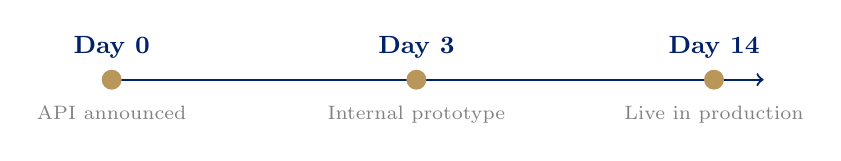
\begin{tikzpicture}[scale=0.9]
  \draw[->, thick, color=primaryblue] (0,0) -- (9.2,0);

  \foreach \x/\label/\sub in {
    0/{Day 0}/{API announced},
    4.3/{Day 3}/{Internal prototype},
    8.5/{Day 14}/{Live in production}
  }{
    \fill[primarygold] (\x,0) circle (4pt);
    \node[font=\small\bfseries\color{primaryblue}, above=4pt] at (\x,0) {\label};
    \node[font=\scriptsize\color{gray}, below=6pt]            at (\x,0) {\sub};
  }
\end{tikzpicture}
\end{center}
\vspace{1em}
\begin{keybox}[]
  \centering
  \small\hi{Speed is a product strategy.}\\
  \footnotesize\neutral{Clarity of purpose, not cleverness of code.}
\end{keybox}
\end{frame}

% --- Slide 17: Proactive Messaging ---
\begin{frame}{Proactive Messaging}
\begin{center}
  {\large\hi{What if AI reached out to YOU?}}\\[0.3em]
  {\normalsize\itshape Before you even asked.}
\end{center}
\vspace{0.8em}
\begin{columns}[c]
  \begin{column}{0.3\textwidth}
    \begin{methodbox}[Calendar]
      \centering\footnotesize
      \textbf{2:00 PM}\\
      Presentation
    \end{methodbox}
  \end{column}
  \begin{column}{0.08\textwidth}
    \begin{center}
      {\large\color{primarygold}$\rightarrow$}
    \end{center}
  \end{column}
  \begin{column}{0.55\textwidth}
    \begin{keybox}[AI Message]
      \footnotesize\itshape
      ``Your presentation is in 2 hours.\\
      Need help with your talking points?''
    \end{keybox}
  \end{column}
\end{columns}
\vspace{0.8em}
\begin{center}
  {\small Context + Calendar\ \higold{$\rightarrow$}\ Proactive Reminder}\\[0.4em]
  {\footnotesize\neutral{System-initiated, context-driven outreach.}}
\end{center}
\end{frame}

% --- Slide 18: The Startup Grind ---
\begin{frame}{The Startup Grind}
\vspace{0.5em}
\begin{description}[labelwidth=2.2cm, leftmargin=2.5cm]
  \item[\hi{Monday}]    Ship a feature.
  \item[\higold{Tuesday}]   It breaks in production.
  \item[\hi{Wednesday}] Fix it while planning the next one.
\end{description}
\vspace{1.2em}
\begin{highlightbox}[]
  \centering
  {\normalsize This is not a complaint.\ \ \hi{This is the job.}}
\end{highlightbox}
\vspace{0.8em}
\begin{center}
  {\small\neutral{In 18 months at Wrtn: more learning than 5 years at a slower org.}}
\end{center}
\end{frame}

% --- Slide 19: What I Got Wrong ---
\begin{frame}{What I Got Wrong}
\begin{columns}[T]
  \begin{column}{0.47\textwidth}
    \begin{highlightbox}[What I built]
      \footnotesize\centering
      Complex layered memory hierarchy\\
      Short-term · Episodic · Semantic\\[0.4em]
      \neutral{\itshape Technically elegant.}
    \end{highlightbox}
  \end{column}
  \begin{column}{0.47\textwidth}
    \begin{keybox}[What users needed]
      \footnotesize\centering
      \hi{``Just tell me what to do next.''}\\[0.4em]
      \positive{Simple. Direct. Clear.}
    \end{keybox}
  \end{column}
\end{columns}
\vspace{0.9em}
\begin{center}
  {\large\negative{$-$3 weeks}}\ \ {\normalsize of team rework.}\\[0.7em]
  {\large\bfseries\hi{User problem $>$ technical solution.}}
\end{center}
\end{frame}

% --- Slide 20: Skills That Actually Mattered ---
\begin{frame}{Skills That Actually Mattered}
\vspace{0.3em}
\begin{center}
\begin{tabular}{p{3.2cm} p{3.4cm} p{3.4cm}}
  \toprule
  \textbf{\neutral{What I Thought}} & \textbf{\hi{What Actually}} & \textbf{\higold{What You}} \\
  \textbf{\neutral{Mattered}}       & \textbf{\hi{Mattered}}      & \textbf{\higold{Should Build}} \\
  \midrule
  PyTorch proficiency & Problem definition    & One deployed project \\[3pt]
  Publications        & Shipping speed        & One user interview   \\[3pt]
  Algorithm knowledge & User empathy          & One metric improved  \\
  \bottomrule
\end{tabular}
\end{center}
\vspace{0.9em}
\begin{keybox}[]
  \centering
  \small Technical skills are the \neutral{entry ticket}.\\
  \hi{Judgment} is the differentiator.
\end{keybox}
\end{frame}

% --- Slide 21: Startup vs. Big Tech ---
\begin{frame}{Startup vs.\ Big Tech — Honest Truth}
\vspace{0.3em}
\begin{center}
\begin{tabular}{p{2.8cm} p{3.0cm} p{3.0cm}}
  \toprule
  & \textbf{\hi{Startup}} & \textbf{\higold{Big Tech}} \\
  \midrule
  Learning speed  & \positive{3--5 yrs in 1 yr}       & Deep but narrow     \\[3pt]
  Salary (US)     & \$90K--\$220K                      & \$200K--\$550K TC   \\[3pt]
  Ownership       & \positive{High, direct}             & Medium              \\[3pt]
  Risk            & \negative{High (90\% fail)}         & Low--Medium         \\[3pt]
  Work hours      & \negative{50--70+ hrs}              & 40--55 hrs          \\
  \bottomrule
\end{tabular}
\end{center}
\vspace{0.8em}
\begin{center}
  {\normalsize\itshape Neither is better.\ \ \hi{It depends on who you are.}}
\end{center}
\end{frame}

% --- Slide 22: How to Think Like a Product Engineer ---
\begin{frame}{How to Think Like a Product Engineer}
\begin{center}
  {\normalsize\hi{Start with the user's problem.}\ \ Everything else is implementation detail.}
\end{center}
\vspace{0.5em}
\begin{center}
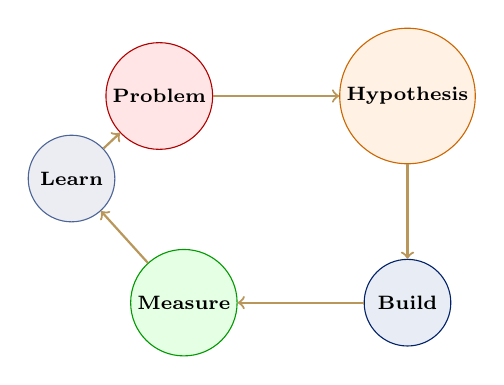
\begin{tikzpicture}[
  node distance=1.2cm and 1.6cm,
  cnode/.style={draw, circle, minimum size=1.1cm, font=\scriptsize\bfseries,
                align=center, inner sep=2pt},
  arr/.style={->, thick, color=primarygold}
]
  \node[cnode, draw=red!70!black,    fill=red!10]     (P) {Problem};
  \node[cnode, draw=orange!80!black, fill=orange!10,  right=of P] (H) {Hypothesis};
  \node[cnode, draw=primaryblue,     fill=lightbg,    below=of H] (B) {Build};
  \node[cnode, draw=green!60!black,  fill=green!10,   left=of B]  (M) {Measure};
  \node[cnode, draw=primaryblue!70,  fill=primaryblue!8, above left=0.7cm and 0.55cm of M] (L) {Learn};

  \draw[arr] (P) -- (H);
  \draw[arr] (H) -- (B);
  \draw[arr] (B) -- (M);
  \draw[arr] (M) -- (L);
  \draw[arr] (L) -- (P);
\end{tikzpicture}
\end{center}
\vspace{0.3em}
\begin{center}
  {\small\itshape Repeat. Forever.}\\[0.4em]
  {\footnotesize\neutral{This is not a startup framework. This is how good engineers everywhere think.}}
\end{center}
\end{frame}

% --- Slide 23: Part 2 Takeaway ---
\begin{frame}[plain]
\begin{center}
\vfill
{\large\itshape\hi{``The 5M users came from problem definition,}}\\[0.5em]
{\large\itshape\hi{not better algorithms.''}}
\vfill
\end{center}
\end{frame}

% ==============================================================================
% PART 3: WoRV STORY (slides 24–35)
% ==============================================================================

% --- Section Divider ---
\begin{frame}[plain]
\begin{center}
\vfill
{\Huge\hi{Leading a Physical AI Research Team}}\\[1em]
{\large\higold{WoRV at Maum.ai}}
\vfill
\end{center}
\end{frame}

% --- Slide 24: Maum.ai WoRV — Three Pillars ---
\begin{frame}{WoRV — World of Robotic Vision}
\vspace{0.5em}
\begin{columns}[T]
  \begin{column}{0.32\textwidth}
    \begin{methodbox}[Navigation]
      \centering
      \vspace{0.3em}
      {\large\hi{Navigation}}\\[0.4em]
      \footnotesize Robots that find their way
    \end{methodbox}
  \end{column}
  \begin{column}{0.32\textwidth}
    \begin{methodbox}[Manipulation]
      \centering
      \vspace{0.3em}
      {\large\hi{Manipulation}}\\[0.4em]
      \footnotesize Robots that use their hands
    \end{methodbox}
  \end{column}
  \begin{column}{0.32\textwidth}
    \begin{methodbox}[Sim / Eval]
      \centering
      \vspace{0.3em}
      {\large\hi{Sim / Eval}}\\[0.4em]
      \footnotesize Infrastructure to prove it works
    \end{methodbox}
  \end{column}
\end{columns}
\vspace{1.2em}
\begin{center}
  {\small\itshape ``I joined as Head of Research in May 2025.''}
\end{center}
\end{frame}

% --- Slide 25: SketchDrive ---
\begin{frame}{SketchDrive: Draw a Map. The Robot Drives It.}
\vspace{0.3em}
\begin{itemize}
  \item Hand-drawn sketch $\rightarrow$ robot navigation route
  \item VLA-based: vision + language + action in one model
  \item \hi{InternVL} backbone: \hi{2$\times$ faster} inference vs.\ alternatives
  \item Data pipeline: \negative{4--5 days} $\rightarrow$ \positive{2--3 hours}
  \item \hi{9 production releases}: v0.1.0 (Jan 2025) $\rightarrow$ v0.2.5 (Jun 2025)
\end{itemize}
\vspace{0.8em}
\begin{keybox}[]
  \footnotesize Source: CANVAS, ICRA 2025 (arXiv:2410.01273) $\cdot$ SketchDrive mono-repo
\end{keybox}
\end{frame}

% --- Slide 26: GINT — pgfplots bar chart ---
\begin{frame}{GINT: Autonomous Agricultural Robot}
\vspace{-0.2em}
\begin{center}
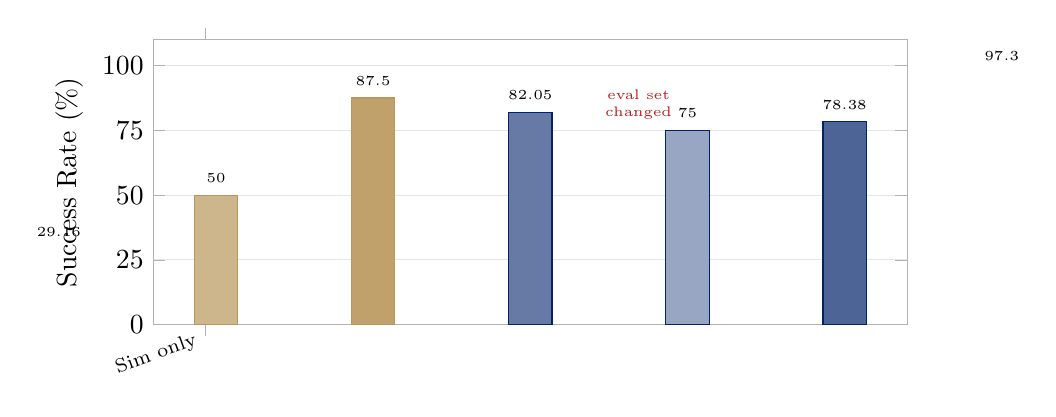
\begin{tikzpicture}
\begin{axis}[
  ybar,
  width=0.92\textwidth,
  height=5.2cm,
  bar width=0.55cm,
  ymin=0, ymax=110,
  ylabel={Success Rate (\%)},
  symbolic x coords={Sim only, +Sim2Real, +Real 2.5h, 1st eval, 2nd eval, 3rd eval, Final},
  xtick=data,
  x tick label style={font=\scriptsize, rotate=20, anchor=east},
  ytick={0,25,50,75,100},
  nodes near coords,
  nodes near coords style={font=\tiny, above},
  every node near coord/.append style={yshift=1pt},
  axis line style={draw=gray!60},
  tick style={draw=gray!60},
  ymajorgrids=true,
  grid style={gray!20},
  enlarge x limits=0.08,
]
  \addplot[fill=negativered!80, draw=negativered] coordinates {
    (Sim only, 29.16)
  };
  \addplot[fill=primarygold!70, draw=primarygold] coordinates {
    (+Sim2Real, 50.00)
  };
  \addplot[fill=primarygold!90, draw=primarygold] coordinates {
    (+Real 2.5h, 87.50)
  };
  \addplot[fill=primaryblue!60, draw=primaryblue] coordinates {
    (1st eval, 82.05)
  };
  \addplot[fill=primaryblue!40, draw=primaryblue] coordinates {
    (2nd eval, 75.00)
  };
  \addplot[fill=primaryblue!70, draw=primaryblue] coordinates {
    (3rd eval, 78.38)
  };
  \addplot[fill=positivegreen!80, draw=positivegreen] coordinates {
    (Final, 97.30)
  };
  % Annotation for the dip
  \node[font=\tiny, text=negativered, align=center] at (axis cs:2nd eval, 85) {eval set\\changed};
\end{axis}
\end{tikzpicture}
\end{center}
\vspace{0.2em}
\begin{center}
  {\small\positive{0\% failure rate at final eval}}\\[0.2em]
  {\small\hi{100+ commercial contracts}, Korea + Japan}
\end{center}
\end{frame}

% --- Slide 27: D2E: Games → Robots ---
\begin{frame}{D2E: Desktop-to-Embodied AI}
\vspace{0.3em}
{\small\itshape Can game recordings teach robots?}
\vspace{0.5em}
\begin{itemize}
  \item \hi{1,300 hours} of game data (1,000h from YouTube)
  \item Collected in \hi{under 1 week} by 1 person
  \item Robot manipulation: \positive{96.6\% success} on LIBERO benchmark
  \item Beats models up to \hi{7$\times$ larger} ($\pi_0$ 3.3B, OpenVLA 7B)
  \item Navigation: \positive{83.3\% success} on CANVAS
\end{itemize}
\vspace{0.8em}
\begin{keybox}[]
  \footnotesize \hi{ICLR 2026 — top 10\%} $\cdot$ Yunsung Lee, corresponding author
\end{keybox}
\end{frame}

% --- Slide 28: Open Source — VLA Eval + OWA ---
\begin{frame}{Open Source Accelerates Everything}
\vspace{0.3em}
\begin{columns}[T]
  \begin{column}{0.50\textwidth}
    \begin{methodbox}[VLA Eval Harness]
      \vspace{0.2em}
      \texttt{vla-eval} (arXiv:2603.13966)\\[0.4em]
      \begin{itemize}\setlength\itemsep{0.2em}
        \item[\footnotesize$\bullet$] \footnotesize \hi{47$\times$} throughput improvement
        \item[\footnotesize$\bullet$] \footnotesize \negative{14h} $\rightarrow$ \positive{18 min} (2,000 LIBERO eps.)
        \item[\footnotesize$\bullet$] \footnotesize \hi{13} benchmarks supported
        \item[\footnotesize$\bullet$] \footnotesize Apache 2.0 — pip installable
      \end{itemize}
    \end{methodbox}
  \end{column}
  \begin{column}{0.47\textwidth}
    \begin{methodbox}[OWA — Open World Agents]
      \vspace{0.2em}
      Desktop agent data framework\\[0.4em]
      \begin{itemize}\setlength\itemsep{0.2em}
        \item[\footnotesize$\bullet$] \footnotesize \hi{400,000} lines of code
        \item[\footnotesize$\bullet$] \footnotesize \hi{226} Pull Requests
        \item[\footnotesize$\bullet$] \footnotesize \hi{1,960} commits
      \end{itemize}
    \end{methodbox}
  \end{column}
\end{columns}
\end{frame}

% --- Slide 29: Infrastructure: CORE Cluster ---
\begin{frame}{CORE: Compute-Oriented Research Environment}
\vspace{0.3em}
DGX H100 cluster — built by the research team.
\vspace{0.5em}

\begin{center}
\small
\begin{tabular}{lccc}
  \toprule
  \textbf{Metric} & \textbf{Before} & \textbf{After} & \textbf{Improvement} \\
  \midrule
  Storage bandwidth & 10\,MB/s & 1\,GB/s & \hi{100$\times$} \\
  Storage capacity  & 28\,TB   & 100\,TB & \hi{3.5$\times$} \\
  Multi-node training & bottlenecked & linear & \hi{$\sim$4$\times$} \\
  \bottomrule
\end{tabular}
\end{center}
\vspace{0.6em}
\begin{center}
  \hi{70,000+} Slurm jobs completed (as of Dec 2025)
\end{center}
\vspace{0.4em}
\begin{keybox}[]
  \footnotesize\itshape ``Good infrastructure is invisible when it works.''
\end{keybox}
\end{frame}

% --- Slide 30: Research Team Culture ---
\begin{frame}{How We Run the WoRV Research Team}
\vspace{0.5em}
\begin{itemize}
  \item \hi{Monthly OKRs} — goals everyone can see and question
  \item \hi{Bi-weekly paper seminars} — what the field is doing
  \item \hi{Daily standups} — what is blocking you right now
  \item \hi{Code review on all research code} — not just production
  \item \hi{1-on-1s every 3 weeks} — career, not just tasks
  \item \hi{Public failure post-mortems} — when evals drop, we discuss why
\end{itemize}
\end{frame}

% --- Slide 31: Researcher Career Paths ---
\begin{frame}{Three Roads into Research}
\vspace{0.2em}
\small
\begin{center}
\begin{tabular}{lccc}
  \toprule
  & \textbf{Academia} & \textbf{Industry Lab} & \textbf{Startup Research} \\
  \midrule
  Freedom          & \positive{Highest} & Medium & \negative{Medium-Low} \\
  Salary           & \negative{Lowest}  & \positive{Highest} & Medium \\
  Impact timeline  & Years  & Months & \positive{Weeks} \\
  Pub.\ pressure   & \negative{Very high} & High & Medium \\
  Job security     & \negative{Low} & Medium & \negative{Low} \\
  What you learn   & Ask new questions & How to scale & \hi{How to ship} \\
  \bottomrule
\end{tabular}
\end{center}
\vspace{0.8em}
\begin{center}
  {\small\itshape\neutral{``None of these is objectively better. Know who you are first.''}}
\end{center}
\end{frame}

% --- Slide 32: Publishing 10+ Papers: Real Tips ---
\begin{frame}{What Actually Gets Papers Accepted}
\vspace{0.2em}
{\small \hi{10+ top-tier publications} (ICLR, CVPR, NeurIPS, ECCV, AAAI, ICRA) $\cdot$ \hi{1,800+ citations}}
\vspace{0.2em}
\begin{enumerate}
  \item \hi{Write the abstract first} — if you can't summarize in 5 sentences, the idea isn't ready
  \item \hi{Think like a reviewer} — every claim needs evidence; every baseline needs a reason
  \item \hi{Pick the right venue} — match your paper's identity to the venue's culture
  \item \hi{Iterate the story}, not just the experiments — a paper is an argument, not a lab report
  \item \hi{Submit early, reject fast} — one rejection cycle = 3--6 months of signal
  \item \hi{Collaborate} with people smarter than you — D2E had 7 co-authors
\end{enumerate}
\end{frame}

% --- Slide 33: Research → Product ---
\begin{frame}{GINT: Lab $\rightarrow$ Field $\rightarrow$ 100+ Farms}
\vspace{0.3em}
\begin{enumerate}
  \item \hi{Simulation research} — Sim2Real method, 29\% $\rightarrow$ 50\%
  \item \hi{Lab prototype} — 87.5\% with 2.5h real data
  \item \hi{Field evaluation} — 4 evals in 8 days, November 2025
  \item \positive{Final result} — \hi{97.3\% success, 0\% failure rate}
  \item \positive{Commercial deployment} — \hi{100+ contracts}, Korea + Japan
\end{enumerate}
\vspace{1em}
\begin{keybox}[]
  \itshape ``Research that doesn't ship is just a hobby.''
\end{keybox}
\end{frame}

% --- Slide 34: Research Engineer Mindset — TikZ Venn Diagram ---
\begin{frame}{The Research Engineer Mindset}
\vspace{0.2em}
\begin{center}
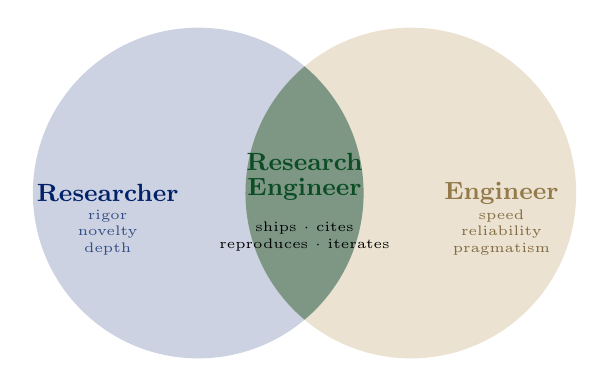
\begin{tikzpicture}
  \begin{scope}[blend mode=multiply]
    % Left circle: Researcher
    \fill[primaryblue!25, opacity=0.8] (-1.35,0) circle (2.1cm);
    % Right circle: Engineer
    \fill[primarygold!35, opacity=0.8] (1.35,0) circle (2.1cm);
    % Overlap: Research Engineer (highlighted)
    \begin{scope}
      \clip (-1.35,0) circle (2.1cm);
      \fill[positivegreen!40, opacity=0.9] (1.35,0) circle (2.1cm);
    \end{scope}
  \end{scope}
  % Labels
  \node[font=\small\bfseries, text=primaryblue] at (-2.5,0) {Researcher};
  \node[font=\tiny, text=primaryblue!80, align=center] at (-2.5,-0.5)
    {rigor\\novelty\\depth};
  \node[font=\small\bfseries, text=primarygold!80!black] at (2.5,0) {Engineer};
  \node[font=\tiny, text=primarygold!70!black, align=center] at (2.5,-0.5)
    {speed\\reliability\\pragmatism};
  \node[font=\small\bfseries, text=positivegreen!60!black] at (0,0.4)
    {Research};
  \node[font=\small\bfseries, text=positivegreen!60!black] at (0,0.05)
    {Engineer};
  \node[font=\tiny, text=black, align=center] at (0,-0.55)
    {ships $\cdot$ cites\\reproduces $\cdot$ iterates};
\end{tikzpicture}
\end{center}
\vspace{0.3em}
\small
\begin{tabular}{l@{\quad+\quad}l}
  Is this true?   & Does this work? \\
  Is this novel?  & Is this fast enough? \\
  Is this rigorous? & Can someone else run it? \\
\end{tabular}
\end{frame}

% --- Slide 35: Part 3 Takeaway ---
\begin{frame}[plain]
\begin{center}
\vfill
{\large\itshape\hi{``Research is still about}}\\[0.5em]
{\large\itshape\hi{solving someone's real problem.''}}
\vfill
\end{center}
\end{frame}

% ==============================================================================
% PART 4: CAREER PREPARATION — THE BLUNT TRUTH (slides 36–55)
% ==============================================================================

% --- Section Divider ---
\begin{frame}[plain]
\begin{center}
\vfill
{\Huge\hi{Career Preparation}}\\[1em]
{\large\higold{The Blunt Truth}}
\vfill
\end{center}
\end{frame}

% ---- 4A: Portfolio & GitHub (Slides 36–40) ----

% --- Slide 36: Your Portfolio Is Your Proof ---
\begin{frame}{Your Portfolio Is Your Proof}
\begin{columns}[c]
  \begin{column}{0.47\textwidth}
    \begin{highlightbox}[Transcript]
      \centering
      {\large\negative{\sout{GPA 3.9}}}\\[0.4em]
      \footnotesize\neutral{Only 4\% of tech leaders\\cite credentials as \#1 signal}
    \end{highlightbox}
  \end{column}
  \begin{column}{0.47\textwidth}
    \begin{keybox}[GitHub]
      \centering
      {\large\positive{Portfolio}}\\[0.4em]
      \footnotesize\positive{\hi{38\%} of tech leaders cite this\\as their \#1 hiring signal}
    \end{keybox}
  \end{column}
\end{columns}
\vspace{1em}
\begin{center}
  {\large\bfseries ``Nobody cares about your GPA.}\\[0.3em]
  {\large\bfseries Show me what you've built.''}
\end{center}
\vspace{0.5em}
{\footnotesize\neutral{Only 23\% cite degree; 17\% cite school prestige; 4\% cite certifications.
Source: Fortune Tech Hiring Secrets, Dec 2025}}
\end{frame}

% --- Slide 37: The Portfolio Skeleton ---
\begin{frame}{The Portfolio Skeleton}
\begin{keybox}[Minimum Viable Portfolio]
  \begin{enumerate}
    \item \hi{GitHub profile} with green contribution squares\\
          {\footnotesize\neutral{Activity $>$ perfection}}
    \item \hi{Tech blog} with 5+ posts\\
          {\footnotesize\neutral{Write about what you build}}
    \item \hi{3 projects} with READMEs and at least one live demo\\
          {\footnotesize\neutral{Deploy at least one}}
  \end{enumerate}
\end{keybox}
\vspace{1em}
\begin{center}
  {\normalsize\itshape ``This is the minimum. Not the ideal.''}\\[0.5em]
  {\small If even one project has a live demo URL — you are ahead of \hi{90\%} of applicants.}
\end{center}
\end{frame}

% --- Slide 38: Good vs. Bad Portfolio ---
\begin{frame}{Good vs.\ Bad Portfolio}
\begin{columns}[T]
  \begin{column}{0.47\textwidth}
    \begin{highlightbox}[Before \negative{$\times$}]
      \footnotesize
      ``Built a calculator app in Java''\\[0.5em]
      \neutral{0 stars\ \textperiodcentered\ no README}\\
      \neutral{last commit 8 months ago}
    \end{highlightbox}
  \end{column}
  \begin{column}{0.47\textwidth}
    \begin{keybox}[After \positive{\checkmark}]
      \footnotesize
      ``Built a RAG chatbot for lecture notes —
      deployed on HuggingFace Spaces,
      1K queries/day,
      Claude API + ChromaDB''\\[0.3em]
      \positive{Live demo\ \textperiodcentered\ recent commits}
    \end{keybox}
  \end{column}
\end{columns}
\vspace{1em}
\begin{center}
  \begin{tabular}{ccc}
    \negative{Vague} & $\rightarrow$ & \positive{Specific} \\[2pt]
    \negative{Local only} & $\rightarrow$ & \positive{Deployed} \\[2pt]
    \negative{No numbers} & $\rightarrow$ & \positive{Metrics} \\
  \end{tabular}
\end{center}
\end{frame}

% --- Slide 39: If Your GitHub Has Only Class Assignments ---
\begin{frame}[plain]
\begin{center}
\vfill
{\large\bfseries ``If your GitHub has only class assignments\ldots''}\\[1em]
{\normalsize you are competing with everyone who also did the homework.}\\[1.5em]
{\LARGE\bfseries\negative{Stand out or get filtered out.}}
\vfill
\end{center}
\end{frame}

% --- Slide 40: What to Build This Month ---
\begin{frame}{What to Build This Month}
\begin{center}
  {\normalsize\bfseries Pick ONE. Ship it. Deploy it. Write about it.}
\end{center}
\vspace{0.6em}
\begin{keybox}[]
  \begin{description}[labelwidth=2.8cm, leftmargin=3.1cm]
    \item[\positive{Beginner}\ (4--8h)] CLI tool with Copilot $\rightarrow$ publish on PyPI
    \item[\higold{Intermediate}\ (6--10h)] Full-stack app with Cursor + v0 $\rightarrow$ deploy on Vercel
    \item[\hi{Advanced}\ (4--6h)] RAG chatbot with Claude API + ChromaDB $\rightarrow$ HuggingFace Spaces
  \end{description}
\end{keybox}
\vspace{0.8em}
\begin{center}
  {\small\itshape All three are free to deploy.
  All three demonstrate production-relevant skills.}
\end{center}
\end{frame}

% ---- 4B: AI Tools as Career Accelerators (Slides 41–44) ----

% --- Slide 41: AI Tools You Must Know ---
\begin{frame}{AI Tools You Must Know}
\begin{center}
  {\fontsize{64}{72}\selectfont\hi{41\%}}\\[0.3em]
  {\normalsize of all code is AI-generated or AI-assisted}\\[0.2em]
  {\footnotesize\neutral{Stack Overflow Developer Survey, 2026}}
\end{center}
\vspace{0.8em}
\begin{center}
  \hi{Claude} \quad\textperiodcentered\quad
  \hi{ChatGPT} \quad\textperiodcentered\quad
  \hi{Cursor} \quad\textperiodcentered\quad
  \hi{Copilot} \quad\textperiodcentered\quad
  \hi{v0}
\end{center}
\vspace{0.8em}
\begin{highlightbox}[]
  \centering
  {\normalsize\bfseries These are not optional anymore.}
\end{highlightbox}
\end{frame}

% --- Slide 42: Build 10x Faster ---
\begin{frame}{Build 10$\times$ Faster}
\begin{columns}[T]
  \begin{column}{0.47\textwidth}
    \begin{highlightbox}[2020]
      \footnotesize\centering
      Full-stack app\\[0.4em]
      \negative{3--4 months}\\[0.3em]
      \neutral{Learn React, Node, Auth,\\CSS, deploy — all from scratch}
    \end{highlightbox}
  \end{column}
  \begin{column}{0.47\textwidth}
    \begin{keybox}[2026]
      \footnotesize\centering
      Same app\\[0.4em]
      \positive{1 weekend}\\[0.3em]
      \positive{v0 generates UI (30 min)\\Cursor adds backend (2 hrs)\\Deploy on Vercel (5 min)}
    \end{keybox}
  \end{column}
\end{columns}
\vspace{1.2em}
\begin{center}
  {\large\bfseries Same app.\ Same quality.\ \hi{10$\times$ faster.}}
\end{center}
\end{frame}

% --- Slide 43: AI for Resume & Interview ---
\begin{frame}{AI for Resume \& Interview}
\begin{center}
  {\large\bfseries ``This is not cheating.''}
\end{center}
\vspace{0.4em}
\begin{enumerate}
  \item \hi{Claude} — paste your resume, ask it to rewrite bullets using STAR with metrics
  \item \hi{ChatGPT} — ``Interview me for an AI engineering role. Ask a medium LeetCode problem.''
  \item \hi{Rezi or Kickresume} — ATS score checker; 75\%+ of resumes are filtered before human review
\end{enumerate}
\vspace{0.4em}
\begin{keybox}[]
  \footnotesize\centering
  Rezi free tier\ \textperiodcentered\ ChatGPT free tier\ \textperiodcentered\ Claude free tier\\
  \neutral{Total cost to overhaul your entire job-search stack: \$0}
\end{keybox}
\end{frame}

% --- Slide 44: Students Who Use AI Ship 10x ---
\begin{frame}{The 10$\times$ Student Framework}
\vspace{0.3em}
\begin{center}
\begin{tabular}{p{4.0cm} p{4.5cm}}
  \toprule
  \textbf{\neutral{Traditional (2020)}} & \textbf{\hi{10$\times$ Student (2026)}} \\
  \midrule
  1--2 projects/year        & \positive{1--2 projects/month} \\[3pt]
  80\% time on boilerplate  & \positive{80\% time on architecture} \\[3pt]
  Limited to studied tech   & \positive{Comfortable with any stack} \\[3pt]
  Portfolio = coursework    & \positive{Portfolio = initiative} \\
  \bottomrule
\end{tabular}
\end{center}
\vspace{1em}
\begin{keybox}[]
  \centering
  \small\hi{AI writes the code.\ You own the understanding.}
\end{keybox}
\end{frame}

% ---- 4C: Resume & Interview Strategy (Slides 45–49) ----

% --- Slide 45: The STAR Method ---
\begin{frame}{The STAR Method}
\begin{center}
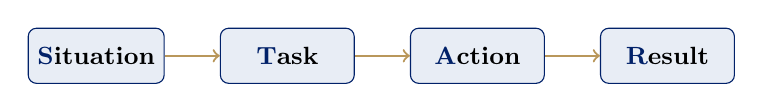
\begin{tikzpicture}[
  node distance=0cm,
  box/.style={draw=primaryblue, fill=lightbg, rounded corners=3pt,
              minimum width=1.7cm, minimum height=0.7cm,
              font=\small\bfseries, align=center},
  arr/.style={->, thick, color=primarygold}
]
  \node[box] (s) {\hi{S}ituation};
  \node[box, right=0.7cm of s] (t) {\hi{T}ask};
  \node[box, right=0.7cm of t] (a) {\hi{A}ction};
  \node[box, right=0.7cm of a] (r) {\hi{R}esult};
  \draw[arr] (s) -- (t);
  \draw[arr] (t) -- (a);
  \draw[arr] (a) -- (r);
\end{tikzpicture}
\end{center}
\vspace{0.7em}
\begin{methodbox}[Real Example — Wrtn]
  \footnotesize
  \textbf{S:} Chatbot had 30\% user drop-off after first session.\\
  \textbf{T:} Reduce drop-off by improving personalization.\\
  \textbf{A:} Built a memory RAG system storing preferences across sessions.\\
  \textbf{R:} Week-1 retention \positive{+12.7\%}.
\end{methodbox}
\vspace{0.5em}
{\footnotesize\negative{``Worked on improving user experience''} vs.\
\positive{``Built memory RAG $\rightarrow$ +12.7\% week-1 retention''}}
\end{frame}

% --- Slide 46: Resume Before → After ---
\begin{frame}{Resume: Before $\rightarrow$ After}
\begin{columns}[T]
  \begin{column}{0.47\textwidth}
    \begin{highlightbox}[\negative{Before $\times$}]
      \footnotesize
      ``Worked on machine learning project''\\[4pt]
      ``Familiar with Python and TensorFlow''\\[4pt]
      ``Participated in data analysis team''
    \end{highlightbox}
  \end{column}
  \begin{column}{0.47\textwidth}
    \begin{keybox}[\positive{After \checkmark}]
      \footnotesize
      ``Built recommendation engine improving CTR by \positive{23\%} for 50K users (PyTorch + Redis)''\\[4pt]
      ``Reduced inference latency \positive{850ms $\rightarrow$ 120ms} via TensorRT''\\[4pt]
      ``Led 3-person pipeline team; data freshness \positive{6h $\rightarrow$ 15min}''
    \end{keybox}
  \end{column}
\end{columns}
\vspace{0.8em}
\begin{center}
  {\small Formula:\ \hi{Built [what] using [tools] resulting in [metric]}}
\end{center}
\end{frame}

% --- Slide 47: Technical Interview Prep — Pyramid ---
\begin{frame}{The Interview Pyramid}
\begin{center}
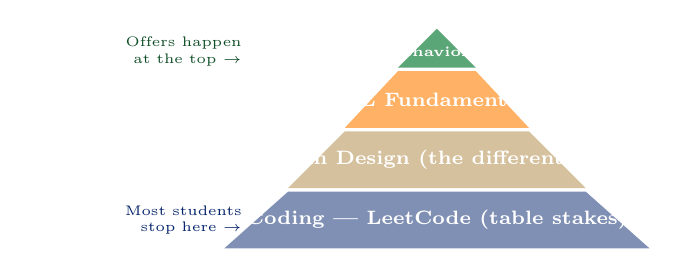
\begin{tikzpicture}[scale=0.9]
  % Layer 1 — bottom: Coding
  \fill[primaryblue!50]  (-3.0,0)    -- (3.0,0)    -- (2.1,0.8)  -- (-2.1,0.8)  -- cycle;
  % Layer 2: System Design
  \fill[primarygold!60]  (-2.1,0.85) -- (2.1,0.85) -- (1.3,1.65) -- (-1.3,1.65) -- cycle;
  % Layer 3: ML Fundamentals
  \fill[orange!60]       (-1.3,1.7)  -- (1.3,1.7)  -- (0.55,2.5) -- (-0.55,2.5) -- cycle;
  % Layer 4 — top: Behavioral
  \fill[positivegreen!70](-0.55,2.55)-- (0.55,2.55)-- (0,3.1)    -- cycle;
  % Labels
  \node[font=\scriptsize\bfseries, text=white]          at (0,    0.4)  {Coding — LeetCode (table stakes)};
  \node[font=\scriptsize\bfseries, text=white]          at (0,    1.25) {System Design (the differentiator)};
  \node[font=\scriptsize\bfseries, text=white]          at (0,    2.1)  {ML Fundamentals};
  \node[font=\tiny\bfseries,       text=white]          at (0,    2.78) {Behavioral};
  % Callouts
  \node[font=\tiny, text=primaryblue, align=right, text width=2.6cm]
        at (-4.2, 0.4)  {Most students\\stop here $\rightarrow$};
  \node[font=\tiny, text=positivegreen!60!black, align=right, text width=2.6cm]
        at (-4.2, 2.78) {Offers happen\\at the top $\rightarrow$};
\end{tikzpicture}
\end{center}
\vspace{0.3em}
{\footnotesize\neutral{LeetCode gets you through the door. System design + ML fundamentals get you the offer.}}
\end{frame}

% --- Slide 48: Culture Fit: What They're Really Asking ---
\begin{frame}{Culture Fit: What They're Really Asking}
\vspace{0.4em}
\begin{description}[labelwidth=5.5cm, leftmargin=5.8cm]
  \item[\textit{``Tell me about a conflict''}]
        = Can you work with humans?
  \item[\textit{``Describe a time you failed''}]
        = Do you take ownership or blame others?
  \item[\textit{``Why this company?''}]
        = Did you spend 30 minutes researching us?
\end{description}
\vspace{1em}
\begin{keybox}[]
  \footnotesize\centering
  Prepare \hi{5 STAR stories} before every interview.\\
  Map them to these question types. Reuse and adapt.
\end{keybox}
\end{frame}

% --- Slide 49: Stop Listing Technologies ---
\begin{frame}{Stop Listing Technologies}
\begin{highlightbox}[\negative{$\times$ Don't Do This}]
  \footnotesize\neutral{Python, TensorFlow, Docker, AWS, PyTorch, React, MongoDB, Redis, Kubernetes, Git}\\[0.3em]
  \footnotesize\neutral{Every CS student lists the same 10 keywords. This tells me nothing.}
\end{highlightbox}
\vspace{0.8em}
\begin{keybox}[\positive{\checkmark} Show, don't list]
  \footnotesize
  ``Deployed a real-time inference pipeline serving \hi{10K req/s} on AWS,\\
  using PyTorch + TensorRT + Redis caching.\\
  Reduced P99 latency from 2.1s to \positive{180ms}.''
\end{keybox}
\vspace{0.8em}
\begin{center}
  {\small Any student can \negative{list} Python.
  Very few can \positive{show} what they built with it.}
\end{center}
\end{frame}

% ---- 4D: What Top Students Are Actually Doing (Slides 50–52) ----

% --- Slide 50: Year-by-Year Roadmap ---
\begin{frame}{Year-by-Year Roadmap}
\vspace{0.3em}
\begin{columns}[T]
  \begin{column}{0.24\textwidth}
    \hi{Year 1: Explore}\\[0.4em]
    \footnotesize
    Python + ML basics\\[2pt]
    First GitHub commits\\[2pt]
    Join one community
  \end{column}
  \begin{column}{0.24\textwidth}
    \hi{Year 2: Build}\\[0.4em]
    \footnotesize
    2 side projects\\[2pt]
    First internship app\\[2pt]
    Start blogging
  \end{column}
  \begin{column}{0.24\textwidth}
    \higold{Year 3: Ship}\\[0.4em]
    \footnotesize
    3 deployed projects\\[2pt]
    AI internship\\[2pt]
    Open source PR
  \end{column}
  \begin{column}{0.24\textwidth}
    \higold{Year 4: Land}\\[0.4em]
    \footnotesize
    Polish portfolio\\[2pt]
    Interview prep\\[2pt]
    Internship $\rightarrow$ FTE
  \end{column}
\end{columns}
\vspace{0.7em}
\begin{center}
  {\small 2+ AI-specific internships = dramatically better outcomes \hi{regardless of GPA}.}\\[0.2em]
  {\footnotesize\neutral{Source: Fortune Tech Hiring Secrets, Dec 2025; ai-job-market research}}
\end{center}
\end{frame}

% --- Slide 51: Networking That Actually Works ---
\begin{frame}{Networking That Actually Works}
\vspace{0.3em}
\begin{tabular}{p{6.0cm} l}
  \toprule
  \textbf{Activity} & \textbf{Effectiveness} \\
  \midrule
  Open Source Contributions  & \positive{$\bigstar\bigstar\bigstar\bigstar\bigstar$} \\[3pt]
  Technical Communities (PR12, TF Korea) & \positive{$\bigstar\bigstar\bigstar\bigstar$} \\[3pt]
  Conferences \& Meetups     & \higold{$\bigstar\bigstar\bigstar$} \\[3pt]
  LinkedIn (active posting)  & \neutral{$\bigstar\bigstar$} \\[3pt]
  Career Fairs               & \neutral{$\bigstar$} \\
  \bottomrule
\end{tabular}
\vspace{0.8em}
\begin{keybox}[]
  \centering
  \small ``Your next job comes from someone who has \hi{seen your work}.''
\end{keybox}
\end{frame}

% --- Slide 52: The 80/20 of Career Prep ---
\begin{frame}{The 80/20 of Career Prep}
\begin{columns}[T]
  \begin{column}{0.47\textwidth}
    \begin{keybox}[\positive{High Impact (20\% of time)}]
      \footnotesize
      \positive{\checkmark} Portfolio projects (deployed)\\[3pt]
      \positive{\checkmark} AI tool fluency\\[3pt]
      \positive{\checkmark} Networking + open source\\[3pt]
      \positive{\checkmark} Interview prep (STAR + LeetCode + system design)
    \end{keybox}
  \end{column}
  \begin{column}{0.47\textwidth}
    \begin{highlightbox}[\negative{Low Impact (80\% of time)}]
      \footnotesize
      \negative{$\times$} Collecting certificates\\[3pt]
      \negative{$\times$} Perfecting GPA 3.7 $\rightarrow$ 3.9\\[3pt]
      \negative{$\times$} Mass-applying without tailoring\\[3pt]
      \negative{$\times$} ``Learning'' without building
    \end{highlightbox}
  \end{column}
\end{columns}
\vspace{0.8em}
\begin{center}
  {\normalsize\bfseries Stop preparing to prepare.\ \hi{Start building.}}
\end{center}
\end{frame}

% ---- 4E: Action Plan (Slides 53–55) ----

% --- Slide 53: 3 Things You Do TODAY ---
\begin{frame}{3 Things You Do TODAY}
\begin{keybox}[Before you leave this room]
  \begin{enumerate}
    \item \hi{Set up your GitHub profile}\\
          {\footnotesize Write a bio. Pin your best repo.
          Apply for the Student Developer Pack (100+ free tools).}
    \item \hi{Install one AI coding tool}\\
          {\footnotesize Cursor, Claude Code, or activate free GitHub Copilot.}
    \item \hi{Pick one project from Slide 40}\\
          {\footnotesize Open a new repo. Write the first line of your README tonight.}
  \end{enumerate}
\end{keybox}
\vspace{0.4em}
\begin{center}
  {\large\bfseries 30 minutes.\ \negative{Tonight.}\ Not tomorrow.}
\end{center}
\end{frame}

% --- Slide 54: The 30-Day Challenge ---
\begin{frame}{The 30-Day Challenge}
\begin{center}
  {\normalsize\bfseries Build one project end-to-end in 30 days.}
\end{center}
\vspace{0.7em}
\begin{center}
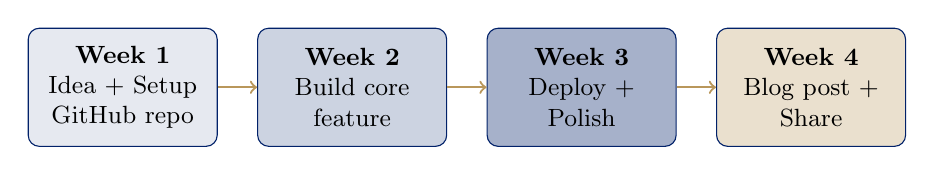
\begin{tikzpicture}[
  box/.style={draw=primaryblue, rounded corners=4pt, fill=lightbg,
              minimum width=2.4cm, minimum height=1.5cm,
              font=\small, align=center},
  arr/.style={->, thick, color=primarygold}
]
  \node[box, fill=primaryblue!10]  (w1) {\textbf{Week 1}\\Idea + Setup\\GitHub repo};
  \node[box, fill=primaryblue!20, right=0.5cm of w1] (w2) {\textbf{Week 2}\\Build core\\feature};
  \node[box, fill=primaryblue!35, right=0.5cm of w2] (w3) {\textbf{Week 3}\\Deploy +\\Polish};
  \node[box, fill=primarygold!30, right=0.5cm of w3] (w4) {\textbf{Week 4}\\Blog post +\\Share};
  \draw[arr] (w1) -- (w2);
  \draw[arr] (w2) -- (w3);
  \draw[arr] (w3) -- (w4);
\end{tikzpicture}
\end{center}
\vspace{0.7em}
\begin{center}
  {\small Day 30 outcome: 1 deployed project\ \textperiodcentered\ 1 blog post\ \textperiodcentered\ updated resume\ \textperiodcentered\ LinkedIn post}\\[0.5em]
  {\normalsize\itshape ``One project. End-to-end. With AI tools.''}
\end{center}
\end{frame}

% --- Slide 55: Your Career Is Yours to Design ---
\begin{frame}[plain]
\begin{center}
\vfill
{\LARGE\bfseries\hi{Your Career Is Yours to Design}}\\[1.5em]
{\normalsize No one else will build your portfolio.}\\[0.4em]
{\normalsize No one else will write your resume.}\\[0.4em]
{\normalsize No one else will show up to your interviews.}\\[1.5em]
{\Large\bfseries\higold{Start now.}}
\vfill
\end{center}
\end{frame}


% ==============================================================================
% PART 5: CLOSING (slides 56–60)
% ==============================================================================

% --- Section Divider: Closing ---
\begin{frame}[plain]
\begin{center}
\vfill
{\Huge\hi{Closing}}\\[1em]
{\large\higold{Your Career Starts Now}}
\vfill
\end{center}
\end{frame}

% --- Slide 56: Recap — AI Landscape ---
\begin{frame}{Recap: The AI Landscape}
\vspace{0.5em}
\begin{center}
\begin{tabular}{@{}ll@{}}
  \hi{\$245K} median AI engineer salary (US) & \higold{50\% of positions unfilled} \\[1.2em]
  \hi{6.1\%} of CS grads unemployed & \higold{Skills mismatch — not supply} \\[1.2em]
  \hi{\$6B+} VC into robotics in H1 2025 & \higold{₩10.1T Korea AI budget (+206\%)} \\
\end{tabular}
\end{center}
\vspace{1.2em}
\begin{center}
  {\normalsize\itshape The demand has never been higher.
  The kind of talent companies need has never been more specific.}
\end{center}
\end{frame}

% --- Slide 57: Recap — My Stories ---
\begin{frame}{Recap: Two Jobs, One Lesson}
\vspace{0.3em}
\begin{tabular}{@{}ll@{}}
  {\fontsize{28}{32}\selectfont\bfseries\hi{5,000,000}} & monthly active users \\[0.9em]
  {\fontsize{28}{32}\selectfont\bfseries\higold{+12.7\%}} & week-1 retention from one RAG feature \\[0.9em]
  {\fontsize{28}{32}\selectfont\bfseries\hi{97.3\%}} & success rate --- up from 29\% \\[0.9em]
  {\fontsize{28}{32}\selectfont\bfseries\higold{ICLR 2026}} & top 10\% --- with game data, not robot data \\[0.9em]
\end{tabular}
\vspace{0.8em}
\begin{center}
  {\normalsize\itshape ``Two jobs. One lesson: problem definition beats algorithms.''}
\end{center}
\end{frame}

% --- Slide 58: Recap — Your Action Plan ---
\begin{frame}{Your Action Plan}
\vspace{0.5em}
\begin{tabular}{@{}lp{8cm}@{}}
  {\large\bfseries\hi{Portfolio}} & Build it. Deploy it. Quantify it. \\[1.2em]
  {\large\bfseries\higold{AI Tools}} & Claude, Cursor, v0. Use them now. Ship 10$\times$ faster. \\[1.2em]
  {\large\bfseries\hi{Networking}} & PR12, open source, LinkedIn. Your next job is a person, not a job board. \\[1.5em]
\end{tabular}
\vspace{0.5em}
\begin{center}
  {\Large\bfseries\higold{Start today, not tomorrow.}}
\end{center}
\end{frame}

% --- Slide 59: Resources & Connect ---
\begin{frame}{Resources \& Connect}
\begin{columns}[T]
  \begin{column}{0.42\textwidth}
    \vspace{0.5em}
    \begin{center}
      \fbox{\parbox[c][4.5cm][c]{3.8cm}{\centering\large QR Code\\[0.5em]\small (resource page)}}\\[0.6em]
      {\small Scan for tools, guides, communities}
    \end{center}
  \end{column}
  \begin{column}{0.55\textwidth}
    \vspace{0.5em}
    \begin{tabular}{@{}ll@{}}
      {\bfseries\hi{LinkedIn}} & \small linkedin.com/in/yunseong-lee \\[0.9em]
      {\bfseries\hi{GitHub}}   & \small github.com/yunseong-lee \\[0.9em]
      {\bfseries\hi{Email}}    & \small yunseong@maum.ai \\[0.9em]
    \end{tabular}
    \vspace{1em}
    {\small\color{gray} Resource list updated quarterly.}
  \end{column}
\end{columns}
\end{frame}

% --- Slide 60: Don't Leave Without a Plan ---
\begin{frame}[plain]
\begin{center}
\vfill
{\LARGE\bfseries\hi{Don't leave without a plan.}}\\[1.5em]
{\large\itshape What is ONE thing you will do this week?}\\[1.5em]
{\normalsize Write it down. Right now.}\\[0.4em]
{\normalsize On your phone. On paper. Anywhere.}\\[1.5em]
{\Large\bfseries\higold{I'll wait.}}
\vfill
\end{center}
\end{frame}

\end{document}
